\documentclass{beamer}
\usepackage[utf8]{inputenc}
\usepackage{graphicx, epsfig}
\usepackage{amsmath,mathrsfs,amsfonts,amssymb}
\usepackage{floatflt}
\usepackage{epic,ecltree}
\usepackage{mathtext}
\usepackage{fancybox}
\usepackage{fancyhdr}
\usepackage{multirow}
\usepackage{enumerate}
\usepackage{epstopdf}
\usepackage{multicol}
\usepackage{algorithm}
\usepackage[noend]{algorithmic}
\usepackage{tikz}
\usepackage{blindtext}
\usetheme{default}%{Singapore}%{Warsaw}%{Warsaw}%{Darmstadt}
\usecolortheme{default}

\setbeamerfont{title}{size=\Huge}
\setbeamertemplate{footline}[page number]{}

\setbeamertemplate{section in toc}[sections numbered]


\makeatletter
\newcommand\HUGE{\@setfontsize\Huge{35}{40}}
\makeatother    

\setbeamerfont{title}{size=\HUGE}
\beamertemplatenavigationsymbolsempty

% latin bold lower
\newcommand{\ba}{\mathbf{a}} 
\newcommand{\bc}{\mathbf{c}} 
\newcommand{\be}{\mathbf{e}} 
\newcommand{\bff}{\mathbf{f}} % \bf - for bold type
\newcommand{\bg}{\mathbf{g}} 
\newcommand{\bh}{\mathbf{h}} 
\newcommand{\bp}{\mathbf{p}} 
\newcommand{\bq}{\mathbf{q}} 
\newcommand{\bt}{\mathbf{t}} 
\newcommand{\bs}{\mathbf{s}} 
\newcommand{\bu}{\mathbf{u}} 
\newcommand{\bv}{\mathbf{v}} 
\newcommand{\bw}{\mathbf{w}} 
\newcommand{\bx}{\mathbf{x}} 
\newcommand{\by}{\mathbf{y}} 
\newcommand{\bz}{\mathbf{z}} 

% latin bold upper
\newcommand{\bA}{\mathbf{A}} 
\newcommand{\bB}{\mathbf{B}} 
\newcommand{\bC}{\mathbf{C}} 
\newcommand{\bG}{\mathbf{G}} 
\newcommand{\bI}{\mathbf{I}} 
\newcommand{\bJ}{\mathbf{J}} 
\newcommand{\bL}{\mathbf{L}} 
\newcommand{\bM}{\mathbf{M}} 
\newcommand{\bP}{\mathbf{P}}
\newcommand{\bQ}{\mathbf{Q}} 
\newcommand{\bR}{\mathbf{R}} 
\newcommand{\bT}{\mathbf{T}} 
\newcommand{\bU}{\mathbf{U}} 
\newcommand{\bV}{\mathbf{V}} 
\newcommand{\bW}{\mathbf{W}} 
\newcommand{\bX}{\mathbf{X}} 
\newcommand{\bY}{\mathbf{Y}} 
\newcommand{\bZ}{\mathbf{Z}} 

% latin cal upper
\newcommand{\cF}{\mathcal{F}} 
\newcommand{\cG}{\mathcal{G}} 
\newcommand{\cI}{\mathcal{I}} 
\newcommand{\cL}{\mathcal{L}} 
\newcommand{\cM}{\mathcal{M}} 
\newcommand{\cN}{\mathcal{N}} 
\newcommand{\cP}{\mathcal{P}} 
\newcommand{\cS}{\mathcal{S}} 
\newcommand{\cT}{\mathcal{T}} 
\newcommand{\cW}{\mathcal{W}} 
\newcommand{\cX}{\mathcal{X}} 
\newcommand{\cZ}{\mathcal{Z}} 

% latin bb upper
\newcommand{\bbE}{\mathbb{E}} 
\newcommand{\bbI}{\mathbb{I}} 
\newcommand{\bbP}{\mathbb{P}} 
\newcommand{\bbR}{\mathbb{R}} 

% greek bold lower
\newcommand{\bepsilon}{\boldsymbol{\epsilon}} 
\newcommand{\btheta}{\boldsymbol{\theta}} 
\newcommand{\blambda}{\boldsymbol{\lambda}} 
\newcommand{\bpi}{\boldsymbol{\pi}} 
\newcommand{\bmu}{\boldsymbol{\mu}} 
\newcommand{\bsigma}{\boldsymbol{\sigma}} 
\newcommand{\bphi}{\boldsymbol{\phi}} 

% greek bold upper
\newcommand{\bSigma}{\boldsymbol{\Sigma}} 

\DeclareMathOperator*{\argmin}{arg\,min}
\DeclareMathOperator*{\argmax}{arg\,max}

\newcommand{\createdgmtitle}[1]{\title[\hbox to 56mm{Deep Generative Models  \hfill\insertframenumber\,/\,\inserttotalframenumber}]
	{\vspace{1cm} \\ \textbf{Deep Generative Models} \\ {\Huge Lecture #1}}
	\author{Roman Isachenko}
		\institute{
\includegraphics[width=0.7cm]{../utils/aimasterslogo} \LARGE{AI Masters}}
	\date{2024, Summer}
}

\usepackage{tikz}
\usetikzlibrary{arrows,shapes,positioning,shadows,trees}

\newcommand\myfootnote[1]{%
  \tikz[remember picture,overlay]
  \draw (current page.south west) +(1in + \oddsidemargin,0.5em)
  node[anchor=south west,inner sep=0pt]{\parbox{\textwidth}{%
      \rlap{\rule{10em}{0.4pt}}\raggedright\scriptsize \textit{#1}}};}

\newcommand\myfootnotewithlink[2]{%
  \tikz[remember picture,overlay]
  \draw (current page.south west) +(1in + \oddsidemargin,0.5em)
  node[anchor=south west,inner sep=0pt]{\parbox{\textwidth}{%
      \rlap{\rule{10em}{0.4pt}}\raggedright\scriptsize\href{#1}{\textit{#2}}}};}
      
\AtBeginSection[]
      {
      	\begin{frame}{Outline}
      		\tableofcontents[currentsection]
      	\end{frame}
      }
      \AtBeginSubsection[]{
      	\begin{frame}{Outline}
      		\tableofcontents[currentsection,currentsubsection]
      	\end{frame}
}
\createdgmtitle{10}

\usepackage{tikz}

\usetikzlibrary{arrows,shapes,positioning,shadows,trees}
%--------------------------------------------------------------------------------
\begin{document}
%--------------------------------------------------------------------------------
\begin{frame}[noframenumbering,plain]
%\thispagestyle{empty}
\titlepage
\end{frame}
%=======
\begin{frame}{Recap of previous lecture}
	How to evaluate likelihood-free models?
	
	$p(y | \bx)$ -- pretrained image classification model (e.g. ImageNet classifier).
	\begin{block}{What do we want from samples?}
		\begin{itemize}
			\item \textbf{Sharpness}
			\begin{figure}
				\centering
				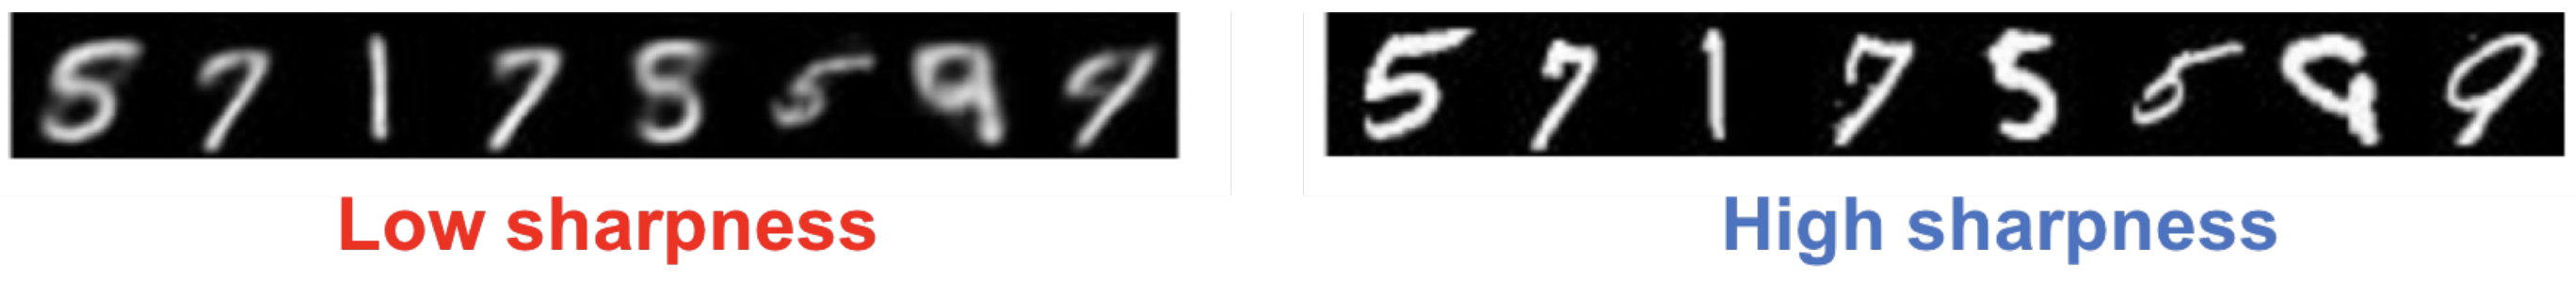
\includegraphics[width=0.9\linewidth]{figs/sharpness}
			\end{figure}
			$p(y | \bx)$ has low entropy (each image $\bx$ should have distinctly recognizable object).
			\item \textbf{Diversity}
			\begin{figure}
				\centering
				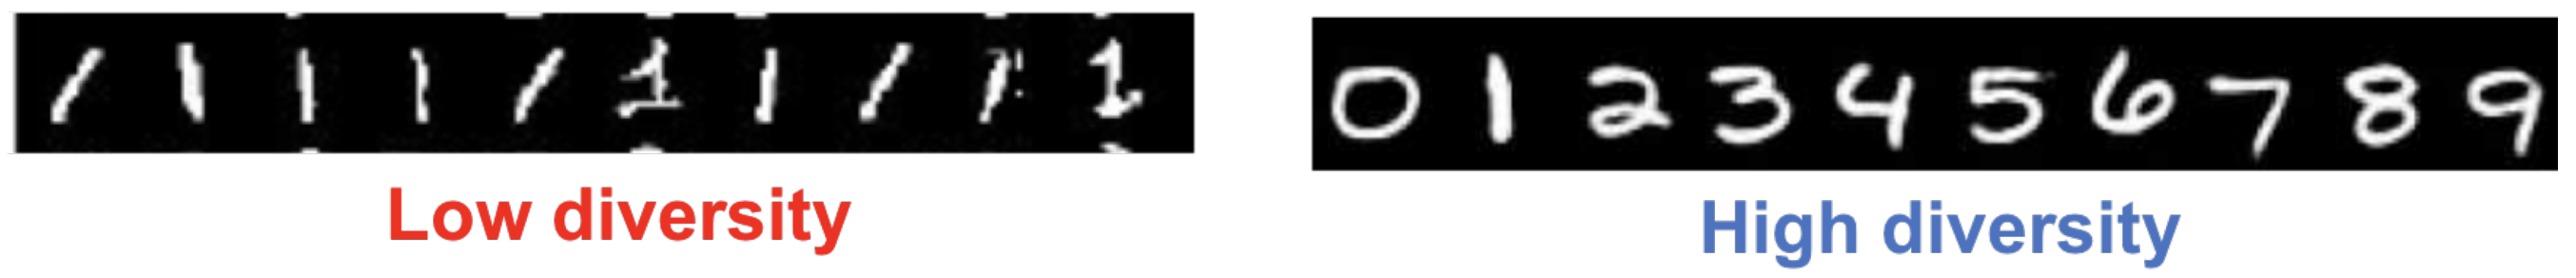
\includegraphics[width=0.9\linewidth]{figs/diversity}
			\end{figure}
			$p(y) = \int p(y | \bx) p(\bx) d \bx$ has high entropy (there should be as many classes generated as possible).
		\end{itemize}
	\end{block}
	\myfootnotewithlink{https://deepgenerativemodels.github.io}{image credit: https://deepgenerativemodels.github.io}
\end{frame}
%=======
\begin{frame}{Recap of previous lecture}
	\vspace{-0.3cm}
	\begin{block}{Frechet Inception Distance (FID)}
		In case of Normal distributions $\pi(\bx) = \cN(\bmu_\pi, \bSigma_\pi)$, $p(\by) = \cN(\bmu_p, \bSigma_p)$:
		\vspace{-0.3cm}
		\begin{multline*}
			\text{FID} (\pi, p) =  W_2^2(\pi, p) = \inf_{\gamma \in \Gamma(\pi, p)} \bbE_{(\bx, \by) \sim \gamma} \| \bx - \by \|^2 \\
			= \| \bmu_{\pi} - \bmu_{p}\|_2^2 + \text{tr} \left[ \bSigma_{\pi} + \bSigma_p - 2 \left(\bSigma_{\pi}^{1/2} \bSigma_p \bSigma_{\pi}^{1/2} \right)^{1/2} \right]
		\end{multline*}
		\vspace{-0.6cm}
	\end{block}		
	\begin{block}{Maximum Mean Discrepancy (MMD)}
		$\pi(\bx) = p(\by)$ if and only if $\bbE_{\pi(\bx)} f(\bx) = \bbE_{p(\by)} f(\by)$ for any bounded and continuous $f$
		\[
			\text{MMD}^2(\pi, p) = \bbE_{\substack{\bx \sim\pi(\bx) \\ \bx' \sim\pi(\bx)}} k(\bx, \bx') + \bbE_{\substack{\by \sim p(\by) \\ \by' \sim p(\by)}} k(\by, \by') - 2 \bbE_{\substack{\bx \sim\pi(\bx) \\ \by \sim p(\by)}} k(\bx, \by)
		\]
	\end{block}		
	
	\myfootnote{\href{https://arxiv.org/abs/1706.08500}{Heusel M. et al. GANs Trained by a Two Time-Scale Update Rule Converge to a Local Nash Equilibrium, 2017} \\
	\href{https://arxiv.org/abs/2401.09603}{Jayasumana S. et al. Rethinking FID: Towards a Better Evaluation Metric for Image Generation, 2024} }
\end{frame}
%=======
\begin{frame}{Recap of previous lecture}
		\begin{itemize}
			\item $\cS_{\pi} = \{\bx_i\}_{i=1}^{n} \sim \pi(\bx)$ -- real samples;
			\item $\cS_{p} = \{\bx_i\}_{i=1}^{n} \sim p(\bx | \btheta)$ -- generated samples.
		\end{itemize}
		Embed samples using pretrained classifier network (as previously):
		\[
			\cG_{\pi} = \{\mathbf{g}_i\}_{i=1}^n, \quad \cG_{p} = \{\mathbf{g}_i\}_{i=1}^n.
		\]
		Define binary function:
		\[
			f(\mathbf{g}, \cG) = 
			\begin{cases}
				1, \text{if exists } \mathbf{g}' \in \cG: \| \mathbf{g}  - \mathbf{g}'\|_2 \leq \| \mathbf{g}' - \text{NN}_k(\mathbf{g}', \cG)\|_2; \\
				0, \text{otherwise.}
			\end{cases}
		\]
		\[
			\text{Precision} (\cG_{\pi}, \cG_{p}) = \frac{1}{n} \sum_{\mathbf{g} \in \cG_{p}} f(\mathbf{g}, \cG_{\pi}); \quad \text{Recall} (\cG_{\pi}, \cG_{p}) = \frac{1}{n} \sum_{\mathbf{g} \in \cG_{\pi}} f(\mathbf{g}, \cG_{p}).
		\]
		\vspace{-0.4cm}
		\begin{figure}
			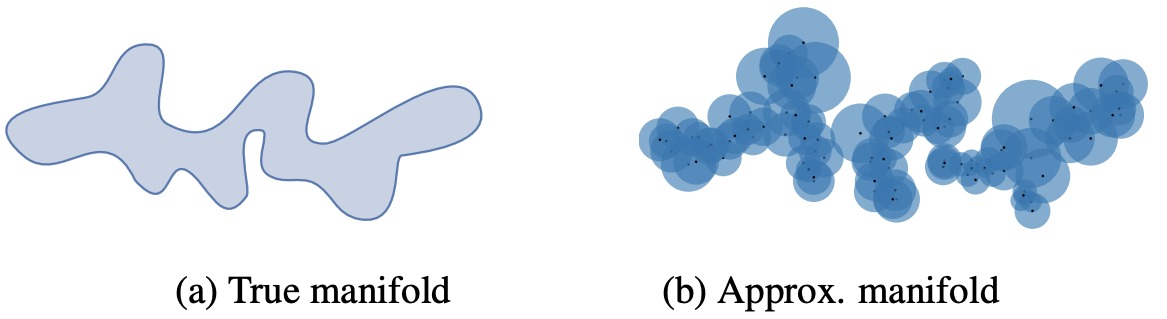
\includegraphics[width=0.7\linewidth]{figs/pr_k_nearest}
		\end{figure}
		\myfootnotewithlink{https://arxiv.org/abs/1904.06991}{Kynkäänniemi T. et al. Improved precision and recall metric for assessing generative models, 2019}
\end{frame}
%=======
\begin{frame}{Recap of previous lecture}
	\begin{block}{Langevin dynamic}
		\vspace{-0.3cm}
		\[
			\bx_{l + 1} = \bx_l + \frac{\eta}{2} \cdot \nabla_{\bx_l} \log p(\bx_l | \btheta) + \sqrt{\eta} \cdot \bepsilon, \quad \bepsilon \sim \cN(0, \bI).
		\]
		\vspace{-0.7cm}
	\end{block}
	\begin{block}{Fisher divergence}
		\vspace{-0.3cm}
		\[
			D_F(\pi, p) = \frac{1}{2}\bbE_{\pi}\bigl\| \nabla_{\bx}\log p(\bx| \btheta) - \nabla_\bx \log \pi(\bx) \bigr\|^2_2 \rightarrow \min_{\btheta}
		\]
		\vspace{-0.7cm}
	\end{block}
	\begin{block}{Score function}
		\vspace{-0.5cm}
		 \[
			 \bs_{\btheta}(\bx) = \nabla_{\bx}\log p(\bx| \btheta)
		 \]
	 \vspace{-0.8cm}
	\end{block}
	\begin{figure}
		\centering
		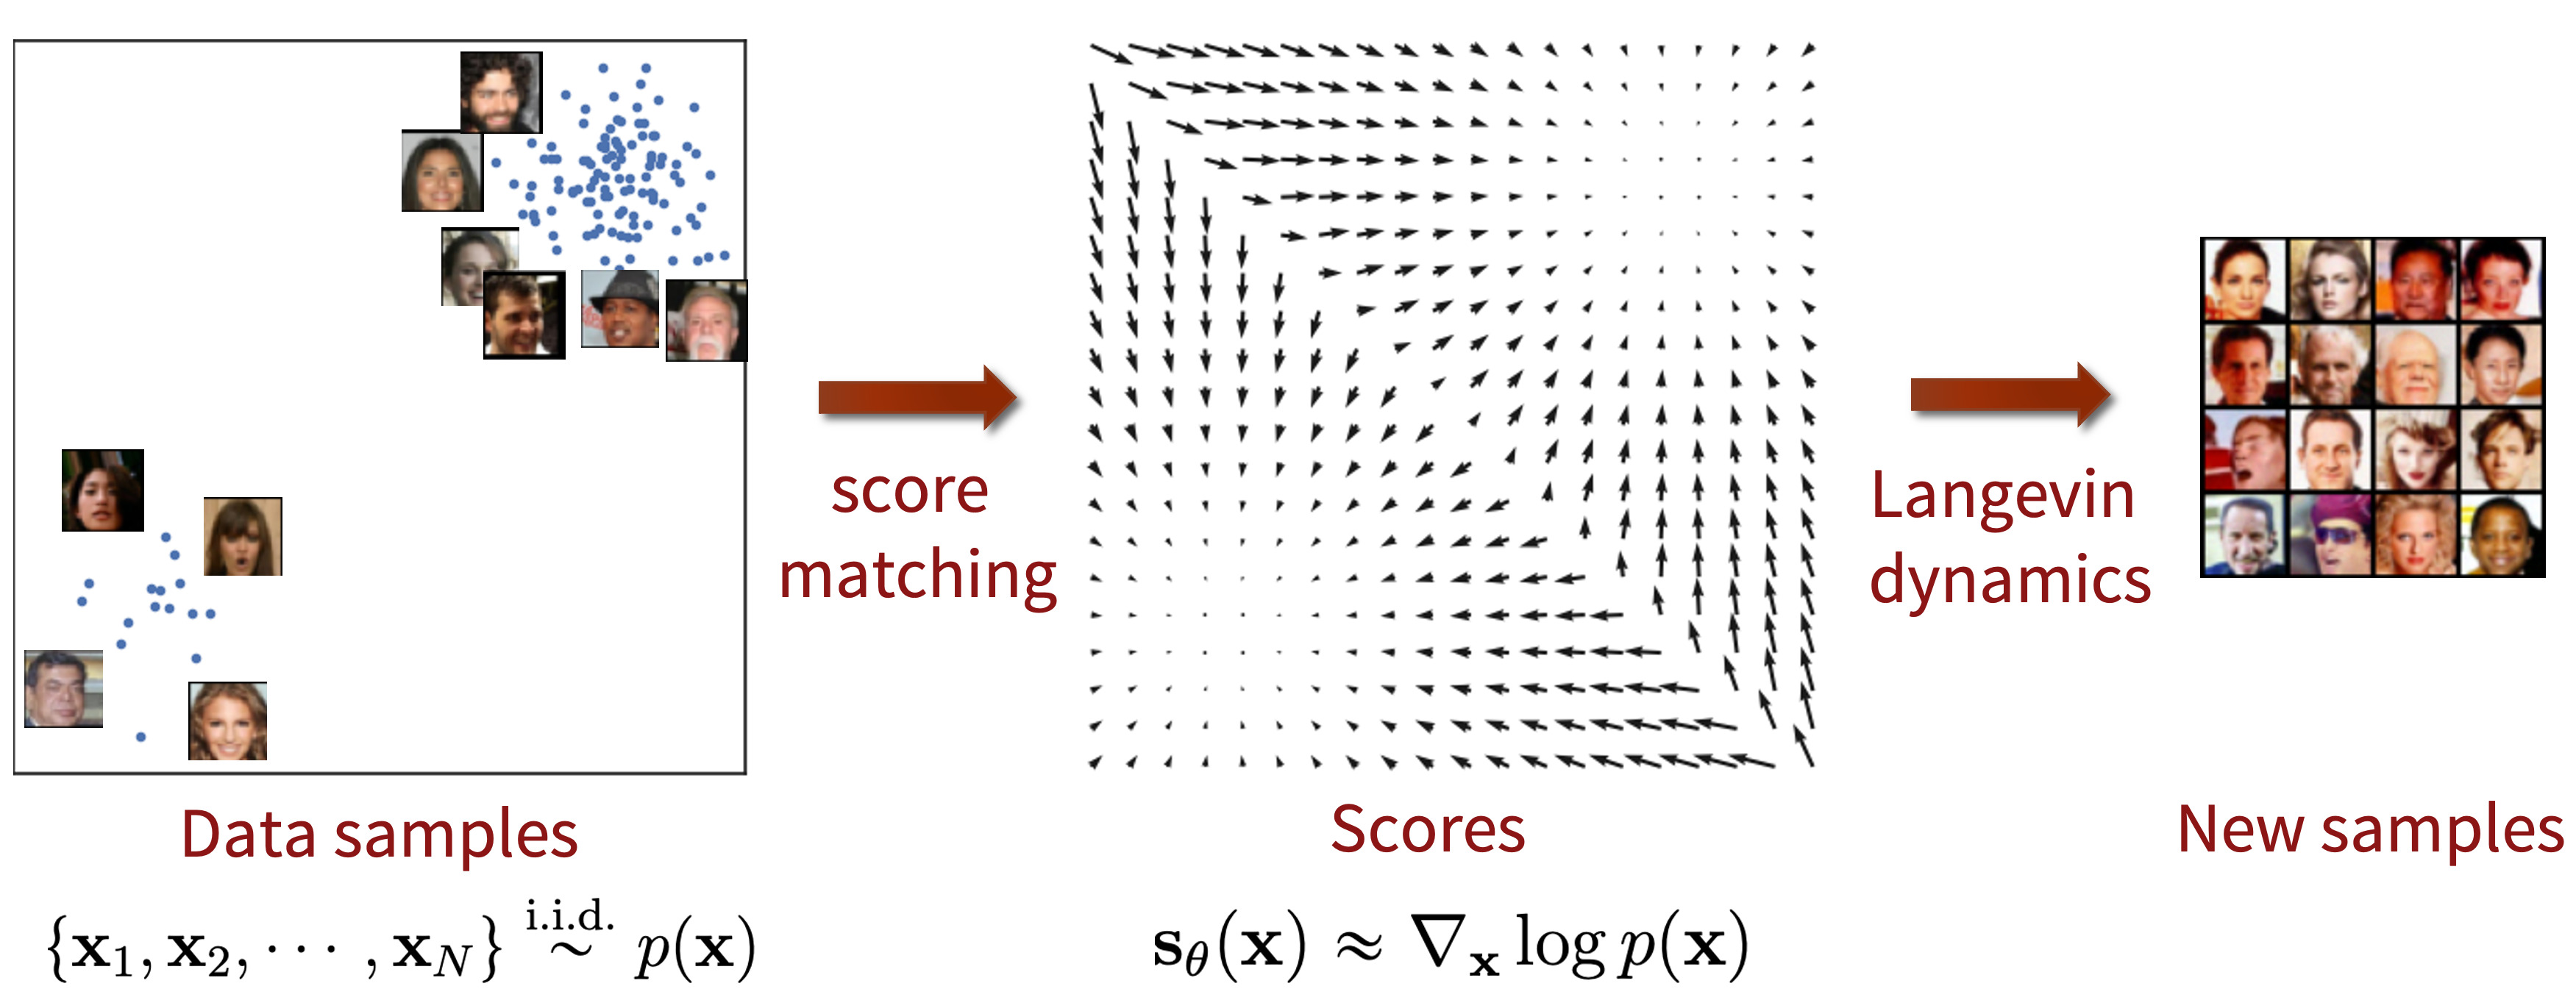
\includegraphics[width=0.75\linewidth]{figs/smld}
	\end{figure}
	\myfootnotewithlink{https://yang-song.github.io/blog/2021/score/}{Song Y. Generative Modeling by Estimating Gradients of the Data Distribution, blog post, 2021}
\end{frame}
%=======
\begin{frame}{Outline}
	\tableofcontents
\end{frame}
%=======
\section{Denoising score matching}
%=======
\begin{frame}{Denoising score matching}
	Let perturb original data $\bx \sim \pi(\bx)$ by random normal noise 
	\[
		\bx_{\sigma} = \bx + \sigma \cdot \bepsilon, \quad \bepsilon \sim \cN(0, \bI), \quad q(\bx_{\sigma} | \bx) = \cN(\bx, \sigma^2 \cdot \bI)
	\]
	\vspace{-0.4cm}
	\[
		q(\bx_{\sigma}) = \int q(\bx_{\sigma} | \bx) \pi(\bx) d\bx.
	\]
	\vspace{-0.4cm} 
	\begin{block}{Assumption}
		The solution of 
		\[
			\frac{1}{2} \bbE_{\pi(\bx_{\sigma} | \sigma)}\bigl\| \bs_{\btheta, \sigma}(\bx_{\sigma}) - \nabla_{\bx_{\sigma}} \log q(\bx_{\sigma}) \bigr\|^2_2 \rightarrow \min_{\btheta}
		\]
		\vspace{-0.3cm} \\
		satisfies $\bs_{\btheta, \sigma}(\bx_{\sigma}) \approx \bs_{\btheta, 0}(\bx_0) = \bs_{\btheta}(\bx)$ if $\sigma$ is small enough.
	\end{block}
	\begin{itemize}
		\item $\bs_{\btheta, \sigma}(\bx_{\sigma})$ tries to \textbf{denoise} a corrupted sample $\bx_{\sigma}$.
		\item Score function $\bs_{\btheta, \sigma}(\bx_{\sigma})$ parametrized by $\sigma$. 
		\item \textbf{Problem:} We don't know $q(\bx_{\sigma})$, just like $\pi(\bx)$.
	\end{itemize}
	\myfootnotewithlink{http://www.iro.umontreal.ca/~vincentp/Publications/smdae_techreport.pdf}{Vincent P. A Connection Between Score Matching and Denoising Autoencoders, 2010}
\end{frame}
%=======
\begin{frame}{Denoising score matching}
	\begin{block}{Theorem}
	\vspace{-0.5cm}
	\begin{multline*}
		\bbE_{q(\bx_{\sigma})}\underbrace{\bigl\| \bs_{\btheta, \sigma}(\bx_{\sigma}) - \nabla_{\bx_{\sigma}} \log q(\bx_{\sigma}) \bigr\|^2_2}_{h(\bx_{\sigma})} = \\
		= \bbE_{\pi(\bx)} \bbE_{q(\bx_{\sigma} | \bx)}\bigl\| \bs_{\btheta, \sigma}(\bx_{\sigma}) - \nabla_{\bx_{\sigma}} \log q(\bx_{\sigma} | \bx) \bigr\|^2_2 + \text{const}(\btheta)
	\end{multline*}
	\vspace{-0.5cm}
	\end{block}
	\begin{block}{Proof}
		\vspace{-0.7cm}
		\begin{multline*}
			\bbE_{q(\bx_{\sigma})} h(\bx_{\sigma}) = \int {\color{violet}q(\bx_{\sigma})} h(\bx_{\sigma}) d\bx_{\sigma} = \\
			= \int \left({\color{violet}\int q(\bx_{\sigma} | \bx) \pi(\bx) d\bx}\right) h(\bx_{\sigma}) d\bx_{\sigma} =  \bbE_{\pi(\bx)} \bbE_{q(\bx_{\sigma} | \bx)}  h(\bx_{\sigma}) d\bx_{\sigma}
		\end{multline*}
		\vspace{-0.7cm}
		{\small
		\begin{multline*}
			\bbE_{q(\bx_{\sigma})}\bigl\| \bs_{\btheta, \sigma}(\bx_{\sigma}) - \nabla_{\bx_{\sigma}} \log q(\bx_{\sigma}) \bigr\|^2_2 = \\ 
			= \bbE_{q(\bx_{\sigma})} \Bigl[\| \bs_{\btheta, \sigma}(\bx_{\sigma}) \|^2 + \underbrace{\| \nabla_{\bx_{\sigma}} \log q(\bx_{\sigma}) \|^2_2}_{\text{const}(\btheta)} - 2 {\color{teal}\bs_{\btheta, \sigma}^T(\bx_{\sigma}) \nabla_{\bx_{\sigma}} \log q(\bx_{\sigma})} \Bigr]
		\end{multline*}
		}
	\end{block}
	\myfootnotewithlink{http://www.iro.umontreal.ca/~vincentp/Publications/smdae_techreport.pdf}{Vincent P. A Connection Between Score Matching and Denoising Autoencoders, 2010}
\end{frame}
%=======
\begin{frame}{Denoising score matching}
	\begin{block}{Theorem}
	\vspace{-0.5cm}
	\begin{multline*}
		\bbE_{q(\bx_{\sigma})}\bigl\| \bs_{\btheta, \sigma}(\bx_{\sigma}) - \nabla_{\bx_{\sigma}} \log q(\bx_{\sigma}) \bigr\|^2_2 = \\
		= \bbE_{\pi(\bx)} \bbE_{q(\bx_{\sigma} | \bx)}\bigl\| \bs_{\btheta, \sigma}(\bx_{\sigma}) - \nabla_{\bx_{\sigma}} \log q(\bx_{\sigma} | \bx) \bigr\|^2_2 + \text{const}(\btheta)
	\end{multline*}
	\vspace{-0.5cm}
	\end{block}
	\begin{block}{Proof (continued)}
		\vspace{-0.7cm}
		{\small
		\begin{multline*}
			\bbE_{q(\bx_{\sigma})} \left[{\color{teal}\bs_{\btheta, \sigma}^T(\bx_{\sigma}) \nabla_{\bx_{\sigma}} \log q(\bx_{\sigma})} \right] = \int q(\bx_{\sigma}) \left[\bs_{\btheta, \sigma}^T(\bx_{\sigma}) \frac{\nabla_{\bx_{\sigma}} {\color{violet}q(\bx_{\sigma})}}{q(\bx_{\sigma})} \right] d\bx_{\sigma} = \\
			= \int \left[\bs_{\btheta, \sigma}^T(\bx_{\sigma}) \nabla_{\bx_{\sigma}}\left({\color{violet}\int q(\bx_{\sigma} | \bx) \pi(\bx) d\bx}\right) \right] d\bx_{\sigma} = \\
			=  \int \int \pi(\bx) \left[\bs_{\btheta, \sigma}^T(\bx_{\sigma}) {\color{olive}\nabla_{\bx_{\sigma}}q(\bx_{\sigma} | \bx)} \right] d\bx_{\sigma} d\bx = \\
			= \int \int \pi(\bx) {\color{olive} q(\bx_{\sigma} | \bx)} \left[\bs_{\btheta, \sigma}^T(\bx_{\sigma}) {\color{olive}\nabla_{\bx_{\sigma}} \log q(\bx_{\sigma} | \bx)} \right] d\bx_{\sigma} d\bx = \\
			= \bbE_{\pi(\bx)} \bbE_{q(\bx_{\sigma} | \bx)} \left[{\color{teal}\bs_{\btheta, \sigma}^T(\bx_{\sigma}) \nabla_{\bx_{\sigma}} \log q(\bx_{\sigma} | \bx)} \right]
		\end{multline*}
		}
	\end{block}
	\myfootnotewithlink{http://www.iro.umontreal.ca/~vincentp/Publications/smdae_techreport.pdf}{Vincent P. A Connection Between Score Matching and Denoising Autoencoders, 2010}
\end{frame}
%=======
\begin{frame}{Denoising score matching}
	\vspace{-0.3cm}
	\begin{block}{Theorem}
	\vspace{-0.7cm}
	\begin{multline*}
		\bbE_{q(\bx_{\sigma})}\bigl\| \bs_{\btheta, \sigma}(\bx_{\sigma}) - \nabla_{\bx_{\sigma}} \log q(\bx_{\sigma}) \bigr\|^2_2 = \\
		= \bbE_{\pi(\bx)} \bbE_{q(\bx_{\sigma} | \bx)}\bigl\| \bs_{\btheta, \sigma}(\bx_{\sigma}) - \nabla_{\bx_{\sigma}} \log q(\bx_{\sigma} | \bx) \bigr\|^2_2 + \text{const}(\btheta)
	\end{multline*}
	\vspace{-0.9cm}
	\end{block}
	\begin{block}{Proof (continued)}
		\vspace{-0.7cm}
		{\small
		\begin{multline*}
			\bbE_{q(\bx_{\sigma})}\bigl\| \bs_{\btheta, \sigma}(\bx_{\sigma}) - \nabla_{\bx_{\sigma}} \log q(\bx_{\sigma}) \bigr\|^2_2 = \\ 
			= {\color{olive}\bbE_{\pi(\bx)} \bbE_{q(\bx_{\sigma} | \bx)}}\Bigl[\| \bs_{\btheta, \sigma}(\bx_{\sigma}) \|^2 - 2 \bs_{\btheta, \sigma}^T(\bx_{\sigma}) {\color{teal}\nabla_{\bx_{\sigma}} \log q(\bx_{\sigma} | \bx)} \Bigr] + \text{const}(\btheta) \\
			= {\color{olive}\bbE_{\pi(\bx)} \bbE_{q(\bx_{\sigma} | \bx)}} \bigl\|\bs_{\btheta, \sigma}(\bx_{\sigma}) - {\color{teal}\nabla_{\bx_{\sigma}} \log q(\bx_{\sigma} | \bx)} \bigr\|_2^2 + \text{const}(\btheta)
		\end{multline*}
		}
		\vspace{-0.8cm}
	\end{block}
	\begin{block}{Gradient of the noise kernel}
	\vspace{-0.3cm}
	\[
		\nabla_{\bx_{\sigma}} \log q(\bx_{\sigma} | \bx) = \nabla_{\bx_{\sigma}} \log \cN(\bx, \sigma^2 \bI) = - \frac{\bx_{\sigma} - \bx}{\sigma^2}  = - \frac{\bepsilon}{\sigma}
	\]
	\vspace{-0.5cm}
	\end{block}
	The RHS does not need to compute $\nabla_{\bx_{\sigma}} \log q(\bx_{\sigma})$ and even $\nabla_{\bx_{\sigma}} \log \pi(\bx_{\sigma})$.
	\myfootnotewithlink{http://www.iro.umontreal.ca/~vincentp/Publications/smdae_techreport.pdf}{Vincent P. A Connection Between Score Matching and Denoising Autoencoders, 2010}
\end{frame}
%=======
\begin{frame}{Denoising score matching}
	Initial objective:
	\vspace{-0.2cm}
	\[
		\bbE_{\pi}\bigl\| \bs_{\btheta}(\bx) - \nabla_\bx \log \pi(\bx) \bigr\|^2_2 \rightarrow \min_{\btheta}
	\]
	\vspace{-0.5cm} \\
	Noised objective:
	\vspace{-0.2cm}
	\[
		\bbE_{\pi}\bigl\| \bs_{\btheta, \sigma}(\bx_\sigma) - \nabla_\bx \log q(\bx_{\sigma}) \bigr\|^2_2 \rightarrow \min_{\btheta}
	\]
	\vspace{-0.5cm} \\
	This is equivalent to denoising task
	\vspace{-0.2cm}
	\[
		\bbE_{\pi(\bx)} \bbE_{q(\bx_{\sigma} | \bx)}\bigl\| \bs_{\btheta, \sigma}(\bx_{\sigma}) - \nabla_{\bx_{\sigma}} \log q(\bx_{\sigma} | \bx) \bigr\|^2_2 \rightarrow \min_{\btheta}
	\]
	\vspace{-0.3cm}
	\[
		\bbE_{\pi(\bx)} \bbE_{\cN(0, \bI)}\left\| \bs_{\btheta, \sigma}(\bx + \sigma \cdot \bepsilon) + \frac{\bepsilon}{\sigma} \right\|^2_2 \rightarrow \min_{\btheta}
	\]
	\vspace{-0.5cm}
	\begin{block}{Langevin dynamic}
		\vspace{-0.3cm}
		\[
			\bx_{l + 1} = \bx_l + \frac{\eta}{2} \cdot \bs_{\btheta, \sigma}(\bx_l) + \sqrt{\eta} \cdot \bepsilon, \quad \bepsilon \sim \cN(0, \bI).
		\]
		\vspace{-0.7cm}
	\end{block}
	\myfootnotewithlink{https://yang-song.github.io/blog/2021/score/}{Song Y. Generative Modeling by Estimating Gradients of the Data Distribution, blog post, 2021}
\end{frame}
%=======
\section{Noise Conditioned Score Network (NCSN)}
%=======
\begin{frame}{Denoising score matching}
	\begin{itemize}
		\item If $\sigma$ is \textbf{small}, the score function is not accurate and Langevin dynamics will probably fail to jump between modes.
		\begin{figure}
			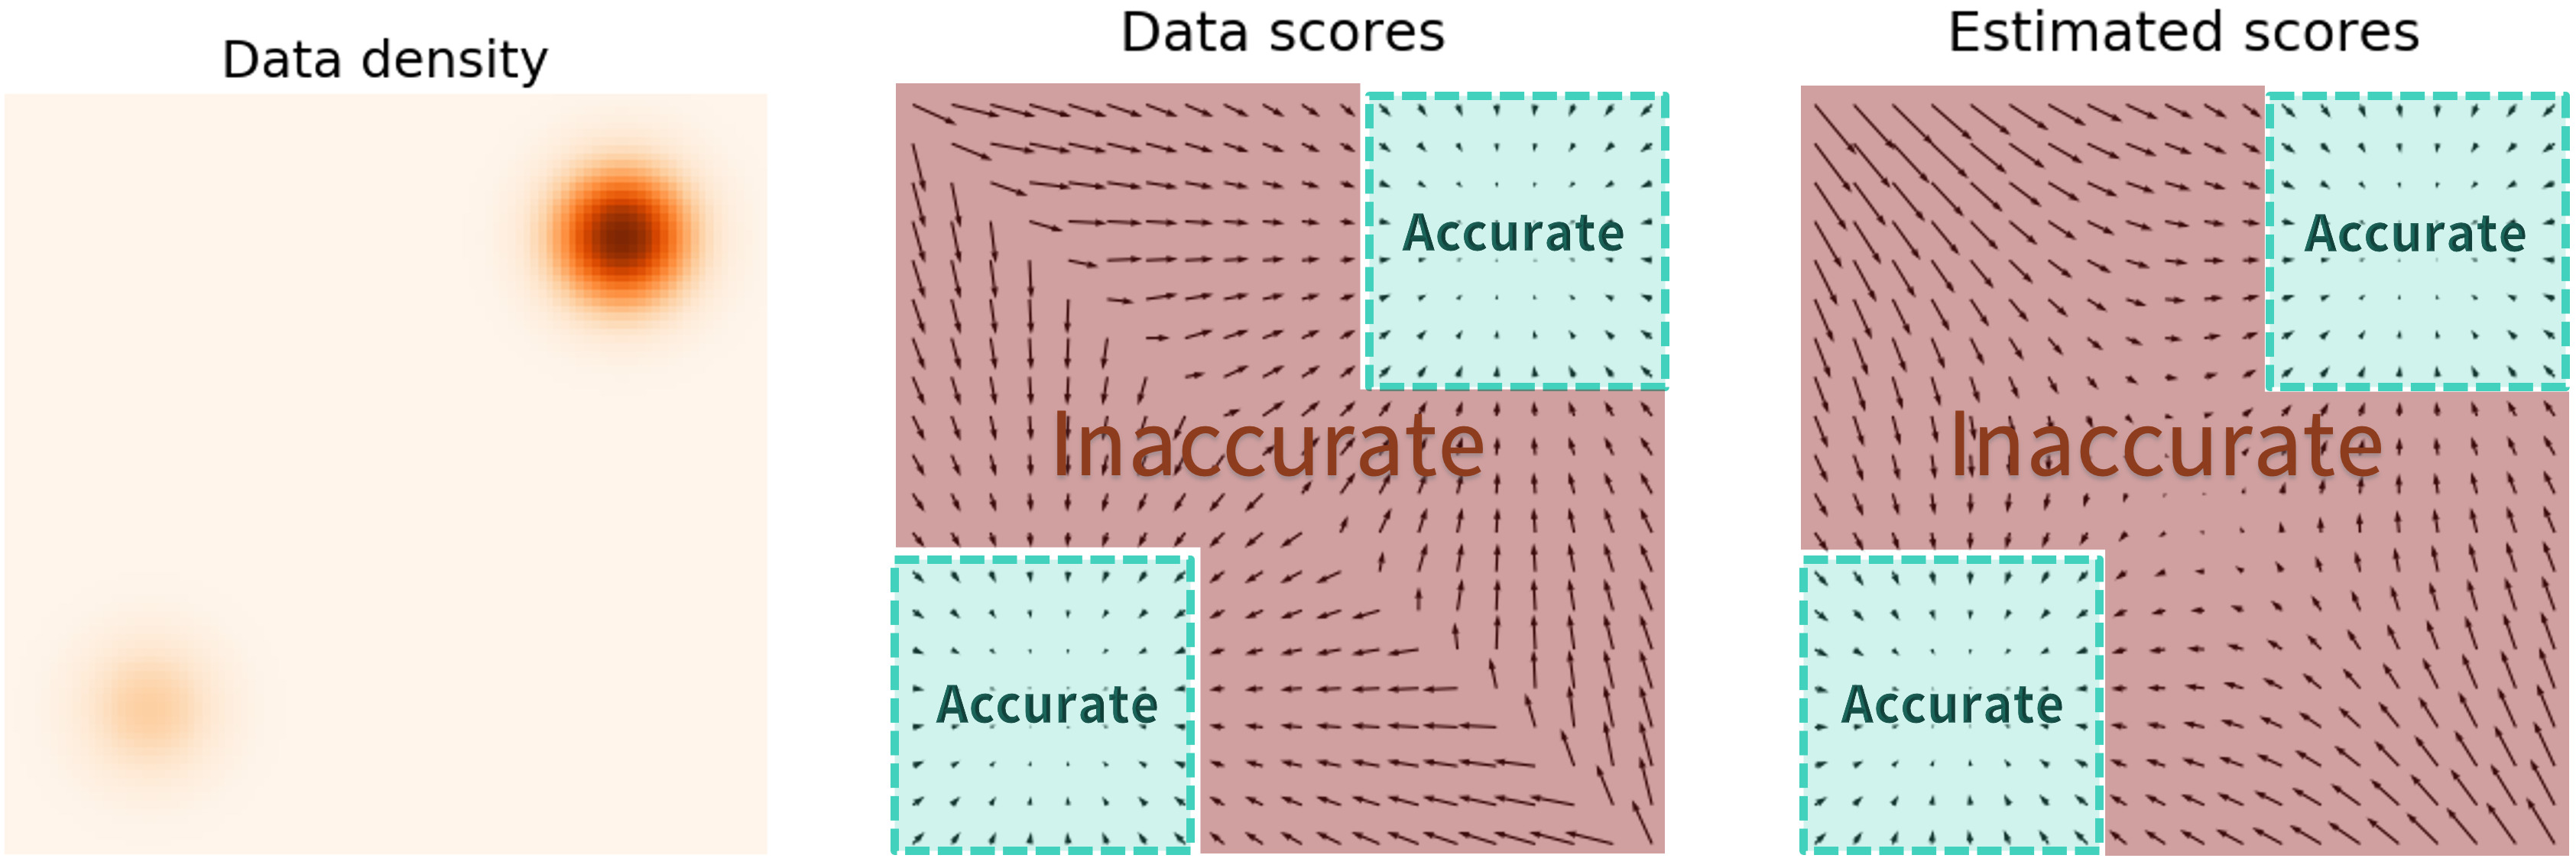
\includegraphics[width=0.75\linewidth]{figs/pitfalls}
		\end{figure}
		\item If $\sigma$ is \textbf{large}, it is good for low-density regions and  multimodal distributions, but we will learn too corrupted distribution.
		\begin{figure}
			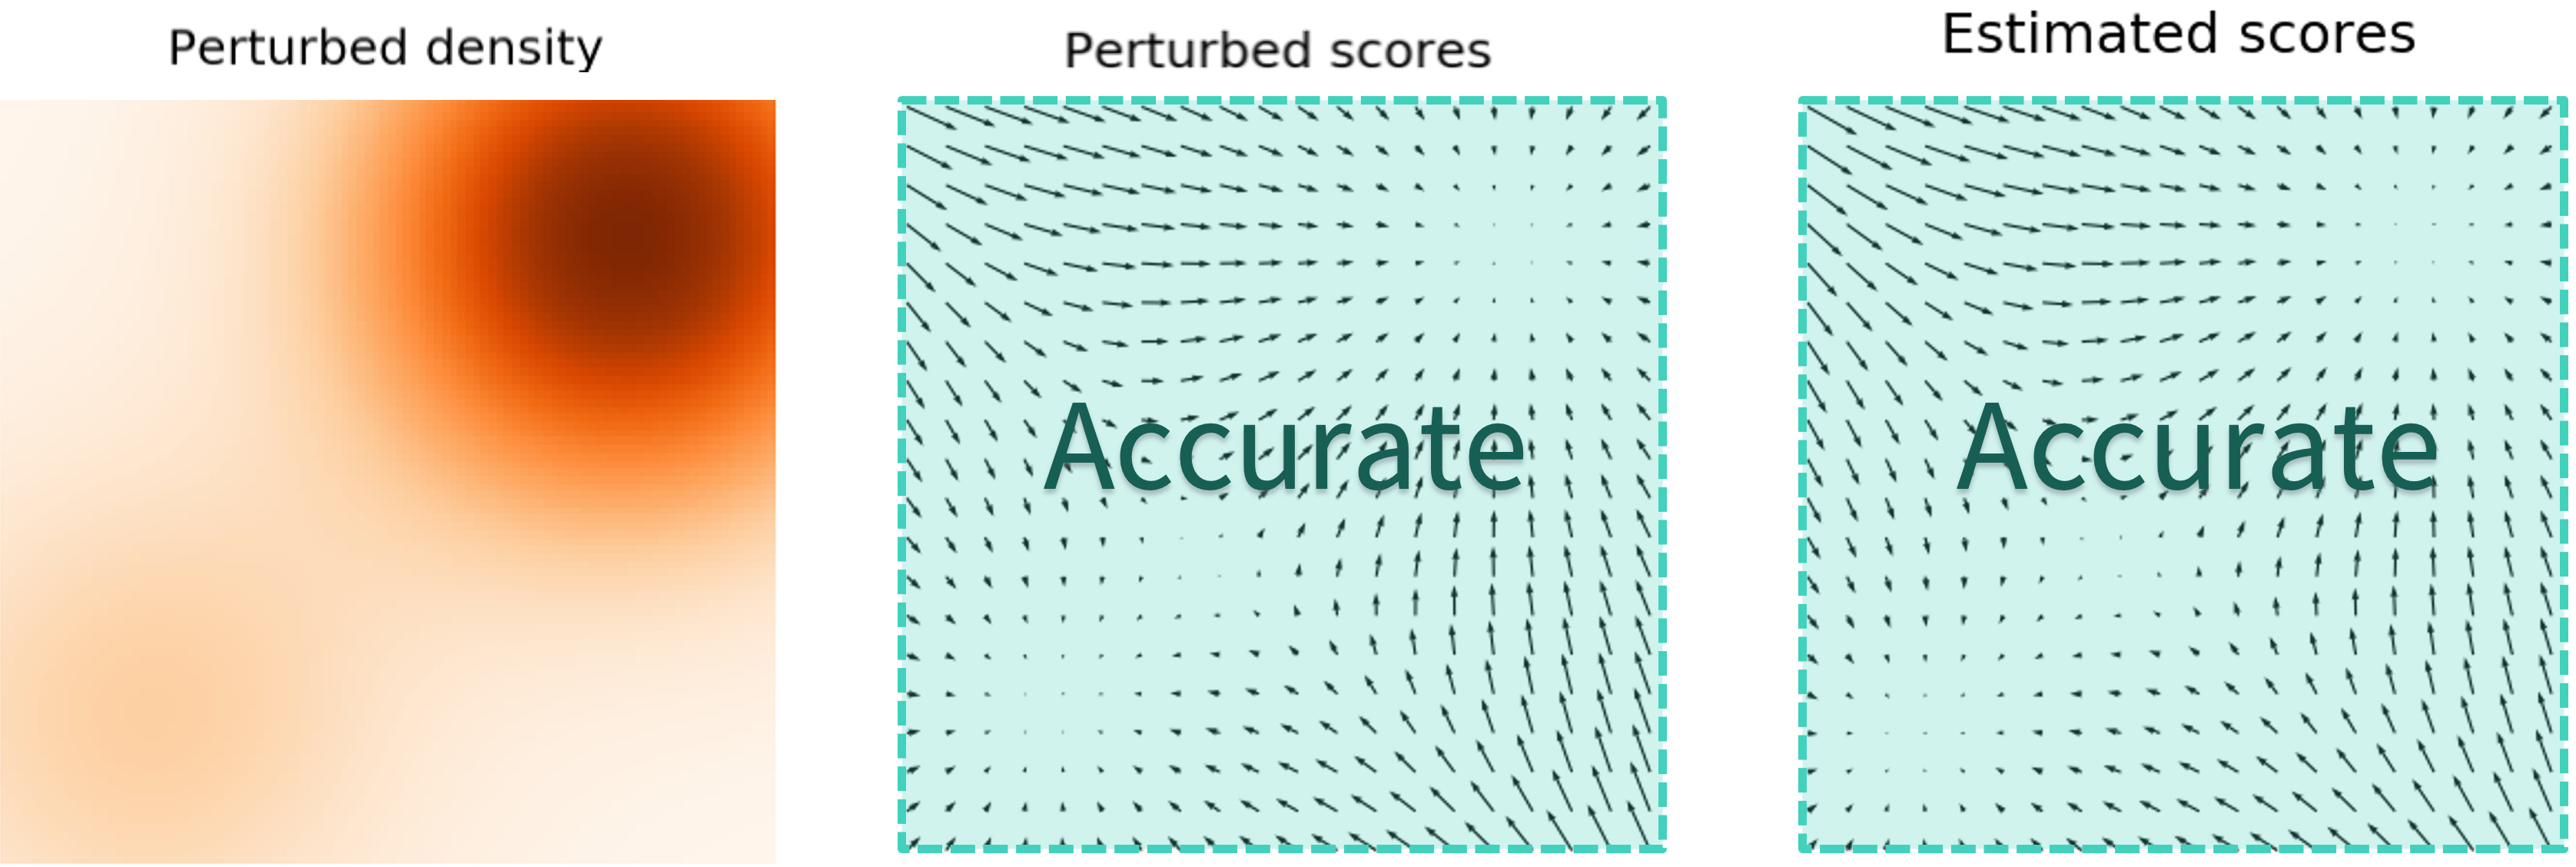
\includegraphics[width=0.75\linewidth]{figs/single_noise}
		\end{figure}
	\end{itemize}
	\myfootnotewithlink{https://yang-song.github.io/blog/2021/score/}{Song Y. Generative Modeling by Estimating Gradients of the Data Distribution, blog post, 2021}
\end{frame}
%=======
\begin{frame}{Noise Conditioned Score Network (NCSN)}
	\begin{itemize}
		\item Define the sequence of the noise levels: $\sigma_1 < \sigma_2 < \dots < \sigma_T$.
		\item Perturb the original data with the different noise levels to obtain $\bx_t = \bx + \sigma_t \cdot \bepsilon$, $\bx_t \sim q(\bx_t)$. 
		\item Choose $\sigma_1, \sigma_T$ such that:
		\[
			q(\bx_1) \approx \pi(\bx), \quad q(\bx_T) \approx \cN(0, \sigma_T^2 \cdot \bI).
		\]
	\end{itemize}
	\begin{figure}
		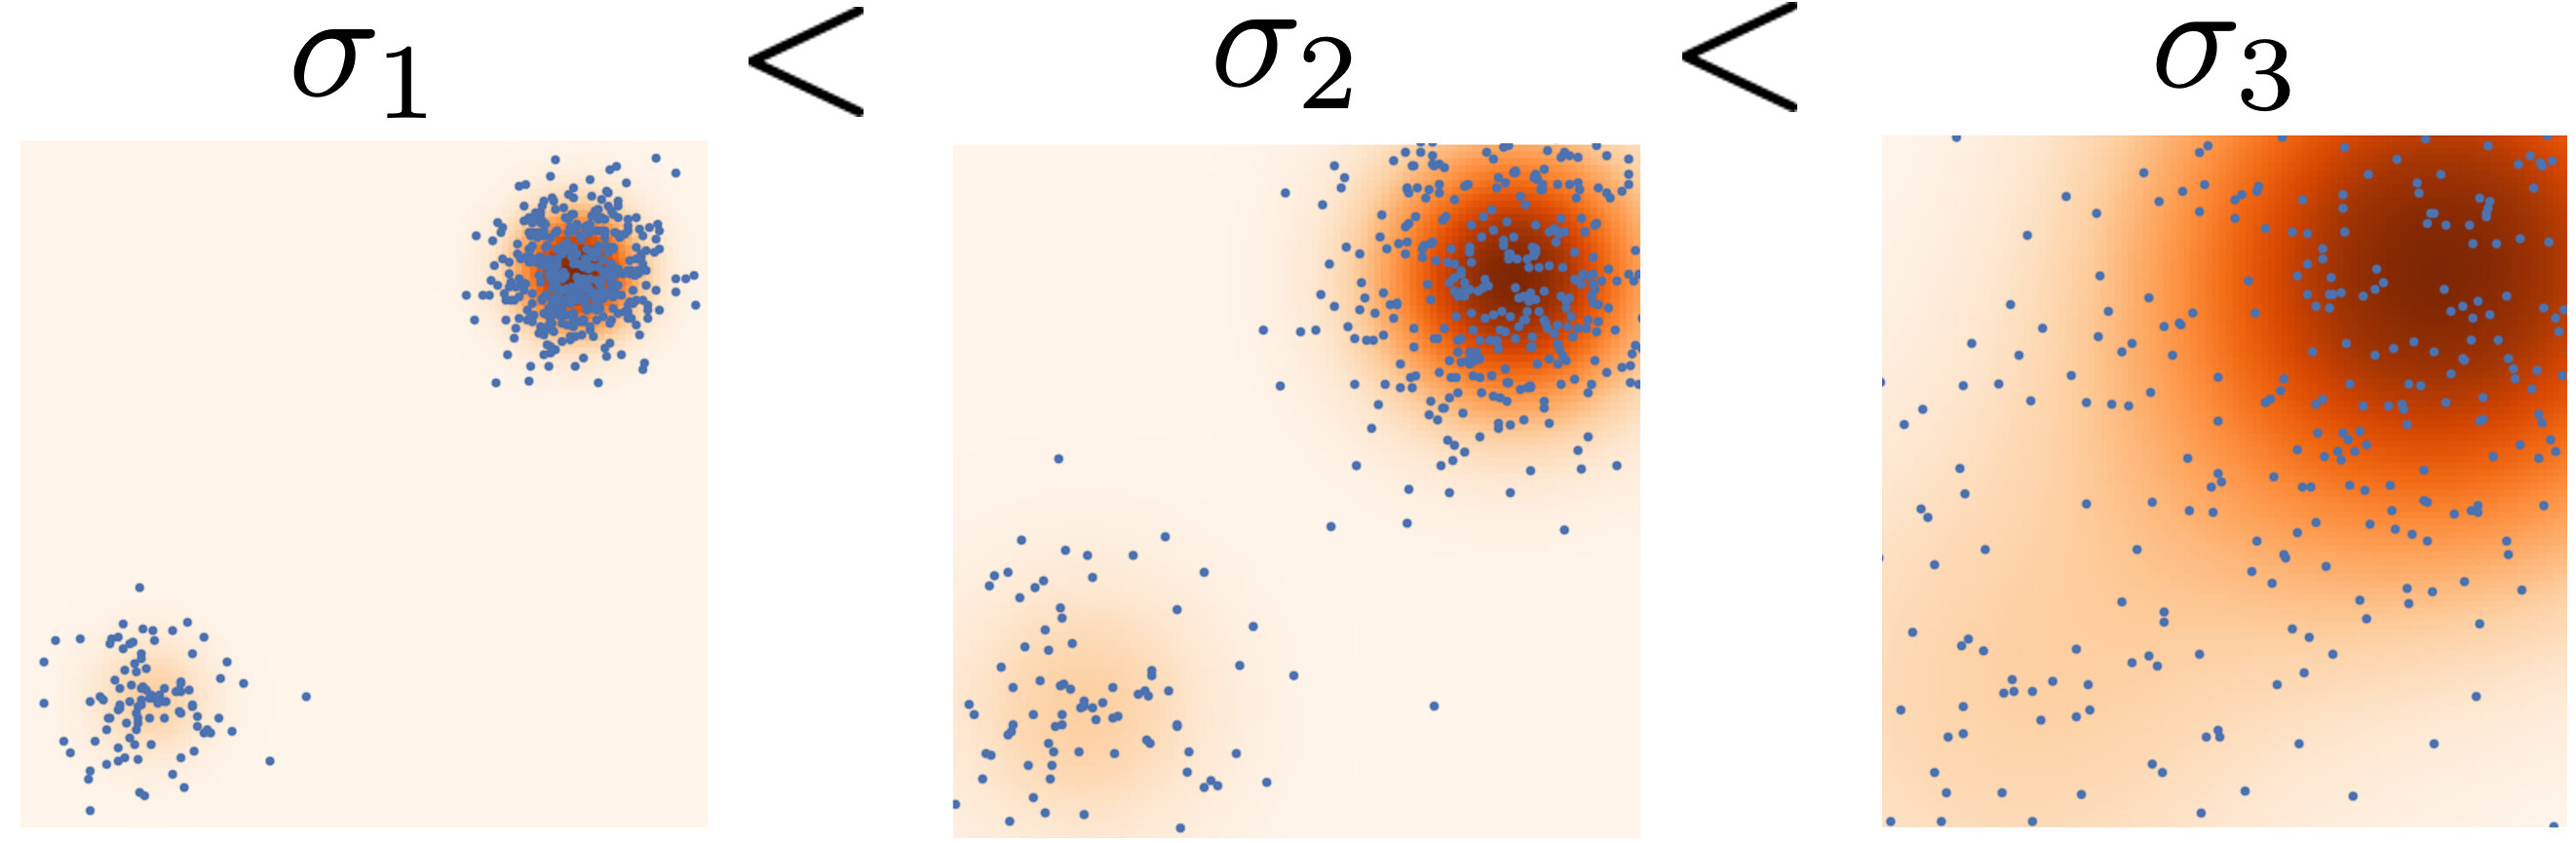
\includegraphics[width=0.6\linewidth]{figs/multi_scale}
	\end{figure}
	\begin{figure}
		
\includegraphics[width=\linewidth]{figs/duoduo}
	\end{figure}
	\myfootnotewithlink{https://arxiv.org/abs/1907.05600}{Song Y. et al. Generative Modeling by Estimating Gradients of the Data Distribution, 2019}
\end{frame}
%=======
\begin{frame}{Noise Conditioned Score Network (NCSN)}
	Train the denoising score function $\bs_{\btheta, \sigma_t}(\bx_t)$ for each noise level using unified weighted objective:
	\vspace{-0.2cm}
	\[
		\sum_{t=1}^T {\color{violet}\sigma_t^2} \cdot \bbE_{\pi(\bx)} \bbE_{q(\bx_t | \bx)}\bigl\| \bs_{\btheta, \sigma_t}(\bx_t) - \nabla_{\bx_t} \log q(\bx_t | \bx) \bigr\|^2_2 \rightarrow \min_{\btheta}
	\]
	Here $\nabla_{\bx_t} \log q(\bx_t | \bx) = - \frac{\bx_t - \bx}{\sigma_t^2} = - \frac{\bepsilon}{\sigma_t}$.
	\begin{block}{Training}
		\begin{enumerate}
			\item Get the sample $\bx_0 \sim \pi(\bx)$.
			\item Sample noise level $t \sim U\{1, T\}$ and the noise $\bepsilon \sim \cN(0, \bI)$.
			\item Get noisy image $\bx_t = \bx_0 + \sigma_t \cdot \bepsilon$.
			\item Compute loss $ \cL = \sigma_t^2 \cdot \| \bs_{\btheta, \sigma_t}(\bx_t) + \frac{\bepsilon}{\sigma_t} \|^2 $.
		\end{enumerate}
	\end{block}
	How to sample from this model?
	\myfootnotewithlink{https://arxiv.org/abs/1907.05600}{Song Y. et al. Generative Modeling by Estimating Gradients of the Data Distribution, 2019}
\end{frame}
%=======
\begin{frame}{Noise Conditioned Score Network (NCSN)}
	\begin{block}{Sampling (annealed Langevin dynamics)}
		\begin{itemize}
			\item Sample $\bx_0 \sim \cN(0, \sigma_T^2 \cdot \bI) \approx q(\bx_T)$.
			\item Apply $L$ steps of Langevin dynamic
			\vspace{-0.2cm}
			\[
				\bx_l = \bx_{l-1} + \frac{\eta_t}{2} \cdot \bs_{\btheta, \sigma_t}(\bx_{l - 1}) + \sqrt{\eta_t} \cdot \bepsilon_l.
			\] 
			\vspace{-0.5cm}
			\item Update $\bx_0 := \bx_L$ and choose the next $\sigma_t$.
		\end{itemize}
	\end{block}
	\begin{figure}
		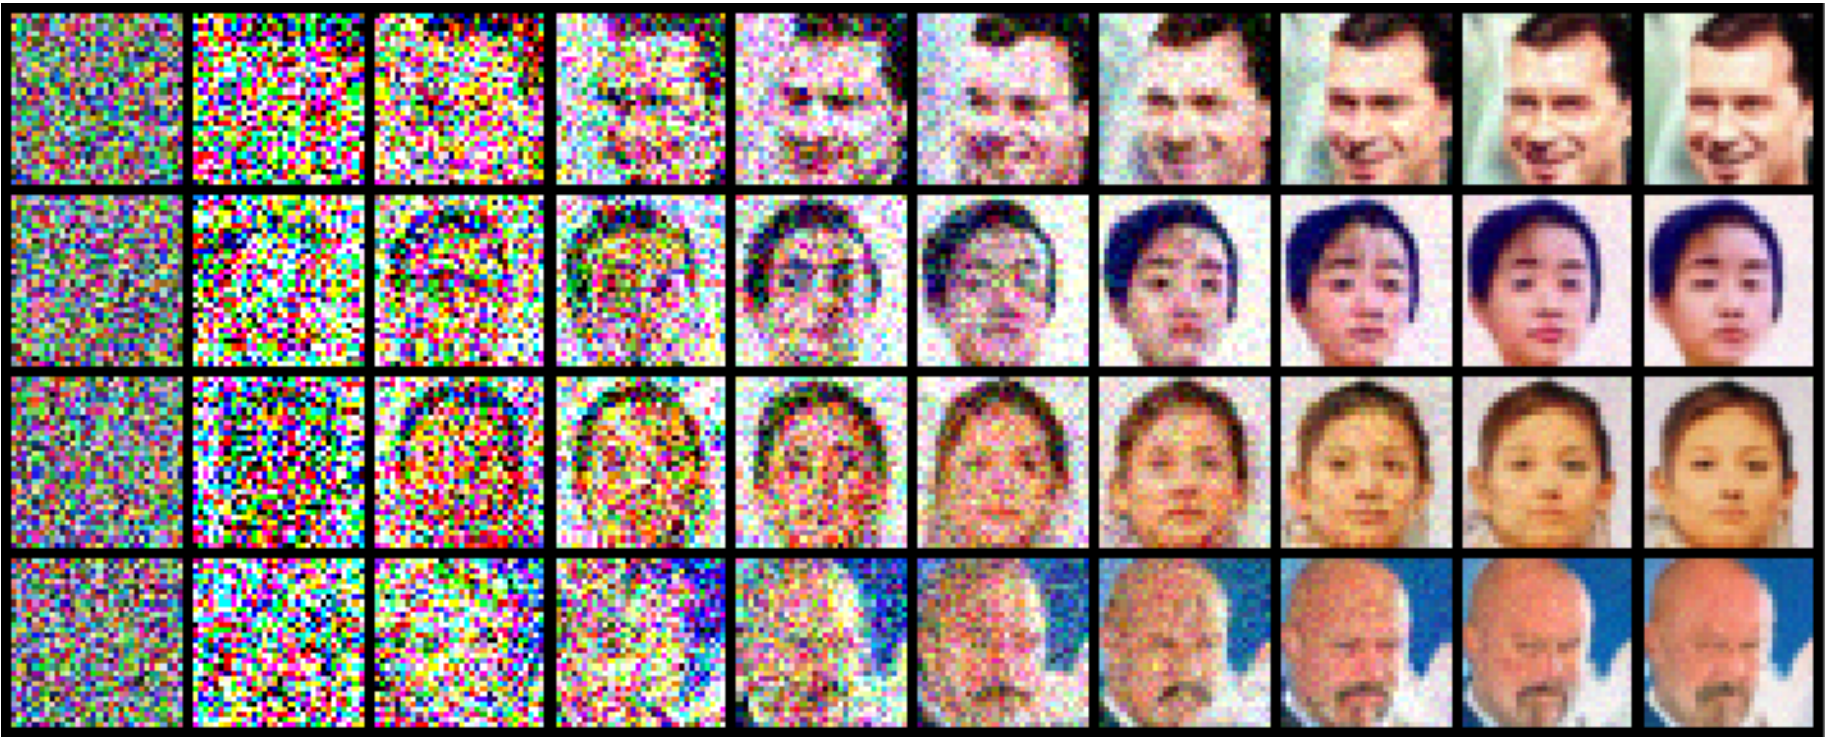
\includegraphics[width=0.9\linewidth]{figs/ald}
	\end{figure}
	\myfootnotewithlink{https://arxiv.org/abs/2006.09011}{Song Y. et al. Improved Techniques for Training Score-Based Generative Models, 2020}
\end{frame}
%=======
\section{Gaussian diffusion process}
%=======
\subsection{Forward gaussian diffusion process}
%=======
\begin{frame}{Forward gaussian diffusion process}
	Let $\bx_0 = \bx \sim \pi(\bx)$, $\beta_t \in (0, 1)$. Define the Markov chain
	\[
		\bx_t = \sqrt{1 - \beta_t} \cdot \bx_{t - 1} + \sqrt{\beta_t} \cdot \bepsilon_t, \quad \text{where }\bepsilon_t \sim \cN(0, \bI);
	\]
	\[
		q(\bx_t | \bx_{t-1}) = \cN(\sqrt{1 - \beta_t} \cdot \bx_{t-1}, \beta_t \cdot \bI).
	\]
	\vspace{-0.5cm}
	\begin{block}{Statement 1}
		Let denote $\alpha_t = 1 - \beta_t$ and $\bar{\alpha}_t = \prod_{s=1}^t \alpha_s = \prod_{s=1}^t (1 - \beta_s)$. Then
		\[
			q(\bx_t | \bx_0) = \cN(\sqrt{\bar{\alpha}_t} \cdot \bx_0, (1 - \bar{\alpha}_t) \cdot \bI)
		\]
		We are able to sample from any timestamp using only $\bx_0$!
		\vspace{-0.2cm}
		{\small
		\begin{multline*}
			\bx_t = \sqrt{\alpha_t} \cdot {\color{teal}\bx_{t-1}} + \sqrt{1 - \alpha_t} \cdot \boldsymbol{\epsilon}_t = \\
			= \sqrt{\alpha_t} ({\color{teal} \sqrt{\alpha_{t-1}} \cdot \bx_{t-2} + \sqrt{1 - \alpha_{t-1}} \cdot  \boldsymbol{\epsilon}_{t-1}}) + \sqrt{1 - \alpha_t} \cdot \boldsymbol{\epsilon}_t = \\
			= \sqrt{\alpha_t \alpha_{t-1}} \cdot \bx_{t-2} + ( {\color{violet}\sqrt{\alpha_t (1 - \alpha_{t-1})} \cdot  \boldsymbol{\epsilon}_{t-1} + \sqrt{1 - \alpha_t} \cdot \boldsymbol{\epsilon}_t}) = \\
			= \sqrt{\alpha_t \alpha_{t-1}} \cdot \bx_{t-2} + {\color{violet}\sqrt{1 - \alpha_{t-1} \alpha_t} \cdot \boldsymbol{\epsilon}'_t} = \\
			 = \dots = \sqrt{\bar{\alpha}_t} \cdot \bx_{0} + \sqrt{1 - \bar{\alpha}_t} \cdot \bepsilon, \quad \text{where } \bepsilon \sim \cN(0, \bI).
		\end{multline*}
		}
	\end{block}
	\myfootnotewithlink{http://proceedings.mlr.press/v37/sohl-dickstein15.pdf}{Sohl-Dickstein J. Deep Unsupervised Learning using Nonequilibrium Thermodynamics, 2015}
 \end{frame}
%=======
\begin{frame}{Forward gaussian diffusion process}
	\vspace{-0.7cm}
	{\small
	\[
		q(\bx_t | \bx_{t-1}) = \cN\left(\sqrt{1 - \beta_t} \bx_{t-1}, \beta_t \bI\right); \quad q(\bx_t | \bx_0) = \cN\left(\sqrt{\bar{\alpha}_t} \bx_0, (1 - \bar{\alpha}_t) \bI\right).
	\]
	}
	\vspace{-0.8cm}
	\begin{figure}
		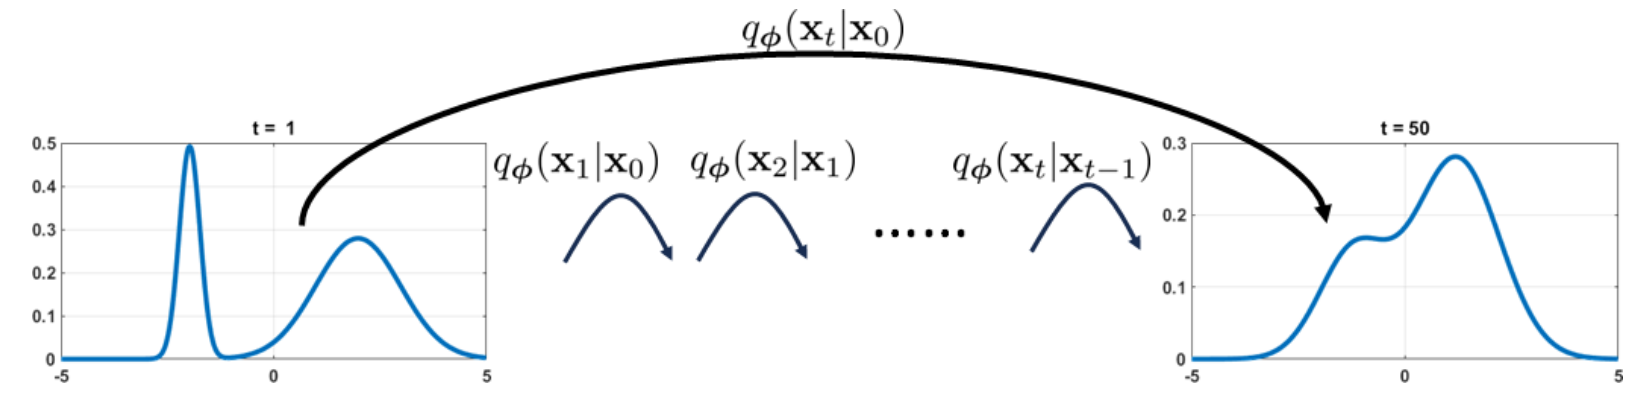
\includegraphics[width=0.8\linewidth]{figs/conditional_diffusion}
	\end{figure}
	\vspace{-0.5cm}
	\begin{block}{Statement 2}
		Applying the Markov chain to samples from any $\pi(\bx)$ we will get $\bx_{\infty} \sim p_{\infty}(\bx) = \cN(0, \bI)$. Here $p_{\infty}(\bx)$ is a \textbf{stationary} and \textbf{limiting} distribution:
		\[
			p_{\infty}(\bx) = \int q(\bx | \bx') p_{\infty}(\bx') d \bx'. 
		\]
		\[
			p_{\infty}(\bx) = \int q(\bx_{\infty} | \bx_0) \pi(\bx_0) d\bx_0 \approx \cN(0, \bI) \int \pi(\bx_0) d\bx_0 = \cN(0, \bI)
		\]
		\vspace{-0.8cm}
	\end{block}
	\myfootnote{\href{https://arxiv.org/abs/2403.18103}{Chan S. Tutorial on Diffusion Models for Imaging and Vision, 2024} \\ \href{http://proceedings.mlr.press/v37/sohl-dickstein15.pdf}{Sohl-Dickstein J. Deep Unsupervised Learning using Nonequilibrium Thermodynamics, 2015}}
 \end{frame}
%=======
\begin{frame}{Forward gaussian diffusion process}
	\textbf{Diffusion} refers to the flow of particles from high-density regions towards low-density regions.
	\vspace{-0.2cm}
	\begin{figure}
		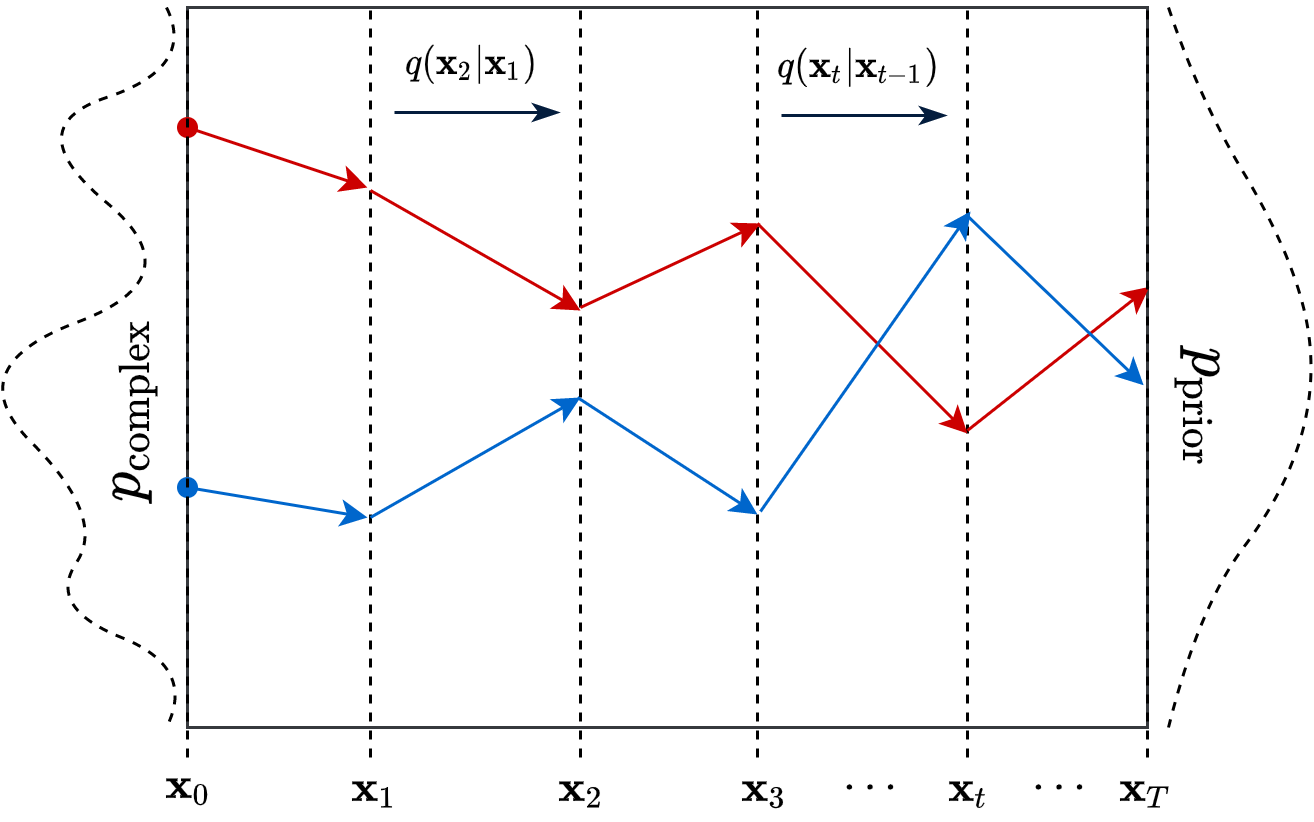
\includegraphics[width=0.5\linewidth]{figs/diffusion_over_time}
	\end{figure}
	\vspace{-0.6cm}
	\begin{enumerate}
		\item $\bx_0 = \bx \sim \pi(\bx)$;
		\item $\bx_t = \sqrt{1 - \beta_t} \cdot \bx_{t - 1} + \sqrt{\beta_t} \cdot \bepsilon$, where $\bepsilon \sim \cN(0, \bI)$, $t \geq 1$;
		\item $\bx_T \sim p_{\infty}(\bx) = \cN(0, \bI)$, where $T >> 1$.
	\end{enumerate}
	If we are able to invert this process, we will get the way to sample $\bx \sim \pi(\bx)$ using noise samples $p_{\infty}(\bx) = \cN(0, \mathbf{I})$. \\ 
	Now our goal is to revert this process.
	\myfootnotewithlink{https://ayandas.me/blog-tut/2021/12/04/diffusion-prob-models.html}{Das A. An introduction to Diffusion Probabilistic Models, blog post, 2021}
\end{frame}
%=======
\subsection{Denoising score matching}
%=======
\begin{frame}{Denoising score matching}
	\begin{block}{NCSN} 
		\vspace{-0.7cm} 
		\[
			\quad q(\bx_t | \bx_0) = \cN(\bx_0, \sigma_t^2 \cdot \bI), \quad q(\bx_1) \approx \pi(\bx), \quad q(\bx_T) \approx \cN(0, \sigma_T^2 \cdot \bI).
		\]
		\[
			\nabla_{\bx_t} \log q(\bx_t | \bx) = - \frac{\bx_t - \bx}{\sigma_t^2}
		\]
		\vspace{-0.6cm} 
	\end{block}
	\begin{block}{Gaussian diffussion}
		\vspace{-0.7cm} 
		\[
			q(\bx_t | \bx_0) = \cN(\sqrt{\bar{\alpha}_t} \cdot \bx_0, (1 - \bar{\alpha}_t) \cdot \bI), \quad q(\bx_1) \approx \pi(\bx), \quad q(\bx_T) \approx \cN(0, \bI)
		\]
		\[
			\nabla_{\bx_t} \log q(\bx_t | \bx_0) = - \frac{\bx_t - \sqrt{\bar{\alpha}_t} \cdot \bx_0}{1 - \bar{\alpha}_t}
		\]
		\vspace{-0.6cm} 
	\end{block}
	\begin{block}{Theorem (denoising score matching)}
	\vspace{-0.7cm}
	\begin{multline*}
		\bbE_{q(\bx_t)}\bigl\| \bs_{\btheta, t}(\bx_t) - \nabla_{\bx_t} \log q(\bx_t) \bigr\|^2_2 = \\
		= \bbE_{\pi(\bx)} \bbE_{q(\bx_t | \bx)}\bigl\| \bs_{\btheta, t}(\bx_t) - \nabla_{\bx_t} \log q(\bx_t | \bx) \bigr\|^2_2 + \text{const}(\btheta)
	\end{multline*}
	\vspace{-0.5cm}
	\end{block}
	\textbf{Note:} We are able to apply NCSN approach with annealed Langevin dynamics to get diffusion denoising model.
\end{frame}
%=======
\begin{frame}{Summary}
	\begin{itemize}
		\item Denoising score matching minimizes Fisher divergence on noisy samples. It allows to estimate Fisher divergence using samples.
		\vfill
		\item Noise conditioned score network uses multiple noise levels and annealed Langevin dynamics to fit score function and sample from the model.	
		\vfill
		\item Gaussian diffusion process is a Markov chain that injects special form of Gaussian noise to the samples.
		\vfill
		\item Denoising score matching is applicable to gaussian diffusion process.
	\end{itemize}
\end{frame}
%=======
\end{document} 